% 原书 p.313–p.322（PDF p.321–p.330）
\section{奇性支撑（I）（Singular Support (I)）}

\begin{keytakeaways}
\begin{itemize}
  \item 几何图像：层的支撑 $\Op{supp}(\mathcal F)$ 太粗糙（例如
        $\mathbf{k}_{(0,2]}$ 与
        $\mathbf{k}_{(0,1]}\oplus\mathbf{k}_{(1,2]}$ 支撑相同但不同构）；
        \textbf{奇性支撑} $SS(\mathcal F)\subset T^*X$ 给出更精细的几何化，
        且与辛几何天然相容。
  \item 数学工具：传播（propagation）的同调判据 (10.33)、奇性支撑的定义
        (10.34)、余法丛 $\nu^*_ZX$（定义 10.6.3）、闭/开区域的余法丛与
        $SS$ 公式（命题 10.6.2）、「锥化」(conification) 技巧 (10.35)–(10.37)。
  \item 本节结论：$SS(\mathbf{k}_Z)=\nu^*_ZX$（子流形情形，命题 10.6.1）；
        拉格朗日子流形与 Hamiltonian 同痕都有层对应物（GKS 层量子化，定理
        10.6.1）。
\end{itemize}
\end{keytakeaways}

% >>> p321
迄今为止，能与 $\mathcal F\in\Op{Ob}(\Op{Sh}(\mathbf{k}_X))$ 相联系的唯一几何
对象是定义 10.2.6 中定义的支撑 $\Op{supp}(\mathcal F)$。然而这种几何化
$\mathcal F\mapsto\Op{supp}(\mathcal F)$ 太粗糙：例如
$\mathbf{k}_{(0,2]}$ 与
$\mathbf{k}_{(0,1]}\oplus\mathbf{k}_{(1,2]}$ 的支撑相同，但由定理 10.2.1，
它们作为 $\R$ 上的可构造层并不同构。因此需要

% >>> p322
更精细的几何化。本节要详细讨论的这种几何化称为\textbf{奇性支撑}
（singular support）：它把一个子集 $SS(\mathcal F)\subset T^*X$（设 $X$ 是
光滑流形）联系到层 $\mathcal F\in\Op{Ob}(\Op{Sh}(\mathbf{k}_X))$（最终可
推广到 $\mathcal F^{\bullet}\in\Op{Ob}(D(\Op{Sh}(\mathbf{k}_X)))$）。注意
$(T^*X,\omega_{\mathrm{can}})$ 是辛流形，因此奇性支撑天然地与辛几何中的各种
要素相互作用。

\begin{wdefn}{10.6.1}（见 [135] 中命题 5.1.1 (1)$_1$ 在层上的应用）
给定层 $\mathcal F\in\Op{Ob}(\Op{Sh}(\mathbf{k}_X))$ 与点
$(x,p)\in T^*X$，称 $\mathcal F$ 在 $(x,p)$ 处\textbf{传播}
（propagates），若对任意函数 $\varphi:X\to\R$（满足 $\varphi(x)=0$ 且
$\dd\varphi(x)=p$），由限制诱导的下述映射
\begin{equation}\tag{10.33}
  \varinjlim_{U\in\operatorname{Op}(X,x)}H^*\bigl(\{\varphi(x)<0\}\cup U;\mathcal F\bigr)
  \to H^*\bigl(\{\varphi(x)<0\};\mathcal F\bigr)
\end{equation}
是层上同调群之间的同构。示意图见图 10.5。
\end{wdefn}

\begin{figure}[htbp]
  \centering
  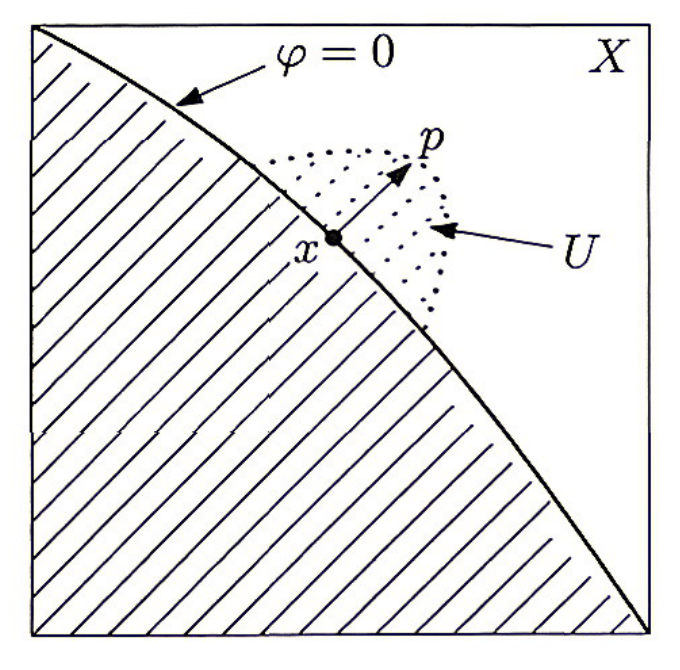
\includegraphics[width=0.44\linewidth]{figures/fig_p322_1.png}
  \caption*{图 10.5\quad 点 $x$ 的一个邻域，其中 $\varphi(x)=0$ 且
  $\dd\varphi(x)=p$（原书 p.314, Figure 10.5）}
\end{figure}

定义 10.6.1 本质上用上同调方法刻画 $\mathcal F$ 能在何处（点 $x\in X$ 的
位置）沿何方向（余向量 $p$）被「延伸」。有时更方便的说法是：$\mathcal F$
在 $(x,p)$ 处\textbf{不}传播，若存在函数 $\varphi:X\to\R$（满足
$\varphi(x)=0$、$\dd\varphi(x)=p$）使得
\[
  \varinjlim_{U\in\operatorname{Op}(X,x)}H^*\bigl(\{\varphi(x)<0\}\cup U;\mathcal F\bigr)
  \quad\text{与}\quad
  H^*\bigl(\{\varphi(x)<0\};\mathcal F\bigr)
\]
\textbf{不}同构。

\begin{wrem}{10.6.1}
由定义 10.6.1 立即可得：若 $\mathcal F$ 在 $(x,p)$ 处传播，则 $\mathcal F$
也在 $(x,\lambda p)$ 处传播（任意 $\lambda>0$）。事实上，只需把检验函数
$\varphi:X\to\R$ 换成 $\lambda\varphi:X\to\R$，则
$\{\lambda\varphi(x)<0\}=\{\varphi(x)<0\}$ 且
$\dd(\lambda\varphi)(x)=\lambda\,\dd\varphi(x)=\lambda p$。
\end{wrem}

\begin{wrem}{10.6.2}
一个远不那么显然的结果是：在定义 10.6.1 中，可以把条件「对任意
$\varphi\cdots$」换成「存在 $\varphi\cdots$」。更多细节见 [135] 中命题
5.1.1。
\end{wrem}
% >>> p323
因此，只需选取一个检验函数，便可验证 $\mathcal F$ 在给定点处是否传播。

为消化定义 10.6.1，我们再次考虑
$\mathbf{k}_{(0,1]}\in\Op{Ob}(\Op{Sh}(\mathbf{k}_{\R}))$，下面的例子考察
$\mathbf{k}_{(0,1]}$ 在何处不传播。

\begin{wexam}{10.6.1}
对每个 $x_0\in\R$，由注 10.6.1，余向量 $p$ 只有 $3$ 种选择：
$p=1$、$p=-1$ 或 $p=0$。对位置 $x\in\R$，有五种不同情形：
\[
  x_0<0,\qquad x_0=0,\qquad x_0\in(0,1),\qquad x_0=1,\qquad x_0>1 .
\]
我们逐类讨论。

(i) 对 $x_0<0$ 与 $p=1$，取 $\varphi(x)=x-x_0$。此时可取 $U$ 为 $x_0$ 附近
的 $(x_0-\epsilon,x_0+\epsilon)$，其中 $\epsilon>0$ 足够小，使得
$x_0+\epsilon<0$。于是检验关系 (10.33) 变为
\[
  \varinjlim_{\epsilon\to0}H^*\bigl((-\infty,x_0+\epsilon);
  \mathbf{k}_{(0,1]}\bigr)
  \to H^*\bigl((-\infty,x_0);\mathbf{k}_{(0,1]}\bigr),
\]
即 $0\to0$。因此 $\mathbf{k}_{(0,1]}$ 在 $(x_0<0,p=1)$ 处传播。类似地，对
$x_0<0$ 与 $p=-1$，取 $\varphi=-x+x_0$，则检验关系 (10.33) 变为
\[
  \varinjlim_{\epsilon\to0}H^*\bigl((x_0-\epsilon,\infty);
  \mathbf{k}_{(0,1]}\bigr)
  \to H^*\bigl((x_0,\infty);\mathbf{k}_{(0,1]}\bigr),
\]
即 $0\to0$。因此 $\mathbf{k}_{(0,1]}$ 在 $(x_0<0,p=-1)$ 处传播。最后，对
$x_0<0$ 与 $p=0$，取 $\varphi\equiv0$，则检验关系 (10.33) 变为
\[
  \varinjlim_{\epsilon\to0}H^*\bigl((x_0-\epsilon,x_0+\epsilon);
  \mathbf{k}_{(0,1]}\bigr)
  \to H^*\bigl(\varnothing;\mathbf{k}_{(0,1]}\bigr),
\]
即 $0\to0$。因此 $\mathbf{k}_{(0,1]}$ 在 $(x_0,p=0)$ 处传播。也可以验证，
对 $(x_0>1,p)$（$p=-1,0,1$）有相同结论。

(ii) 对 $x_0=0$ 与 $p=1$，取 $\varphi(x)=x$，则检验关系 (10.33) 变为
\[
  \varinjlim_{\epsilon\to0}H^*\bigl((-\infty,\epsilon);
  \mathbf{k}_{(0,1]}\bigr)\to H^*\bigl((-\infty,0);
  \mathbf{k}_{(0,1]}\bigr),
\]
即 $0\to0$。因此 $\mathbf{k}_{(0,1]}$ 在 $(0,p=1)$ 处传播。类似地，对
$x_0=0$ 与 $p=-1$，考虑 $\varphi(x)=-x$，则检验关系 (10.33) 变为
\[
  \varinjlim_{\epsilon\to0}H^*\bigl((-\epsilon,\infty);
  \mathbf{k}_{(0,1]}\bigr)\to H^*\bigl((0,\infty);
  \mathbf{k}_{(0,1]}\bigr),
\]
就 $0$ 次上同调群而言这是 $0\to\mathbf{k}$。因此 $\mathbf{k}_{(0,1]}$
\textbf{不}在 $(0,p=-1)$ 处传播。最后，对 $x_0=0$ 与 $p=0$，考虑
$\varphi\equiv0$，则检验关系 (10.33) 变为
\[
  \varinjlim_{\epsilon\to0}H^*\bigl((-\epsilon,\epsilon);
  \mathbf{k}_{(0,1]}\bigr)\to
  H^*\bigl(\varnothing;\mathbf{k}_{(0,1]}\bigr)=0,
\]
% >>> p324
即 $0\to0$。因此 $\mathbf{k}_{(0,1]}$ 在 $(0,p=0)$ 处传播。也可以验证，对
$(x_0=1,p)$ 有类似结论：具体地说，$\mathbf{k}_{(0,1]}$ \textbf{不}在
$(1,p=-1)$ 与 $(1,p=0)$ 处传播，而在 $(1,p=1)$ 处传播。

(iii) 对 $x_0\in(0,1)$ 与 $p=1$，取 $\varphi=x-x_0$，并设 $\epsilon>0$ 足够
小，使得 $x_0+\epsilon<1$ 且 $x_0-\epsilon>0$。则检验关系 (10.33) 变为
\[
  \varinjlim_{\epsilon\to0}H^*\bigl((-\infty,x_0+\epsilon);
  \mathbf{k}_{(0,1]}\bigr)
  \to H^*\bigl((-\infty,x_0);\mathbf{k}_{(0,1]}\bigr),
\]
即 $\mathbf{k}\xrightarrow{\mathbf{1}_{\mathbf{k}}}\mathbf{k}$。因此
$\mathbf{k}_{(0,1]}$ 在 $(x_0,p=1)$ 处传播。类似地，对 $x_0\in(0,1)$ 与
$p=-1$，考虑 $\varphi=-x+x_0$，则检验关系 (10.33) 变为
\[
  \varinjlim_{\epsilon\to0}H^*\bigl((x_0-\epsilon,\infty);
  \mathbf{k}_{(0,1]}\bigr)
  \to H^*\bigl((x_0,\infty);\mathbf{k}_{(0,1]}\bigr),
\]
即 $\mathbf{k}\xrightarrow{\mathbf{1}_{\mathbf{k}}}\mathbf{k}$。因此
$\mathbf{k}_{(0,1]}$ 在 $(x_0,p=-1)$ 处传播。最后，对 $x_0\in(0,1)$ 与
$p=0$，考虑 $\varphi\equiv0$，则检验关系 (10.33) 变为
\[
  \varinjlim_{\epsilon\to0}H^*\bigl((x_0-\epsilon,x_0+\epsilon);
  \mathbf{k}_{(0,1]}\bigr)\to
  H^*\bigl(\varnothing;\mathbf{k}_{(0,1]}\bigr),
\]
就 $0$ 次上同调群而言这是 $\mathbf{k}\to0$。因此 $\mathbf{k}_{(0,1]}$
\textbf{不}在 $(x_0,p=0)$ 处传播。

把上述结果汇总，见图 10.6。\hfill$//$
\end{wexam}

\begin{figure}[htbp]
  \centering
  
\includegraphics[width=0.86\linewidth]{figures/fig_p324_1.png}
  \caption*{图 10.6\quad $T^*\R$ 上的传播点
  （原书 p.316, Figure 10.6）}
\end{figure}

% [Tutor Note: 易错预警——(10.33) 中的极限是对 $x$ 的所有开邻域 $U$ 取
% 正向极限（$\varinjlim$），不是反向极限；被比较的两个上同调群分别是
% 「半空间 $\{\varphi(x)<0\}$ 与 $U$ 的并」和「半空间本身」。$\varphi$ 的
% 选取只需满足 $\varphi(x)=0$、$\dd\varphi(x)=p$（注意这里的 $\varphi$ 是
% 普通函数，其微分取值等于余向量 $p$），不同 $\varphi$ 给出的结论一致
% （注 10.6.2）。例 10.6.1 中所有「$H^*(\cdot;\mathbf{k}_{(0,1]})$」都可以
% 换成「$H^*(\cdot;\mathbf{k})$」来计算，因为所取的区间都落在 $(0,1]$ 或
% 完全避开它。]

\begin{wdefn}{10.6.2}（[135] 中定义 5.1.2 的层版本）
给定层 $\mathcal F\in\Op{Ob}(\Op{Sh}(\mathbf{k}_X))$，$\mathcal F$ 的
\textbf{奇性支撑}定义为
\begin{equation}\tag{10.34}
  SS(\mathcal F):=\overline{\bigl\{(x,p)\in T^*X
  \ \big|\ \mathcal F\ \text{在}\ (x,p)\ \text{处不传播}\bigr\}} .
\end{equation}
\end{wdefn}

由注 10.6.1 与定义 10.6.2 可知，奇性支撑 $SS(\mathcal F)\subset T^*X$ 总是
闭的，并且是\textbf{锥形}的：$\R_{>0}$ 通过缩放余向量分量作用在
$SS(\mathcal F)$ 上。

\begin{wrem}{10.6.3}
在某些文献中，奇性支撑 $SS(\mathcal F)$ 称为\textbf{微支撑}
（micro-support），记为 $\mu S(\mathcal F)$；而在另一些文献中，
$\mu S(\mathcal F)$ 表示 $SS(\mathcal F)$ 模去 $\R_{>0}$-作用后的约化（等价
于把 $SS(\mathcal F)$ 与 $\{p=1\}$ 相交）。
\end{wrem}

% >>> p325
\begin{wexam}{10.6.2}
继续例 10.6.1，我们计算 $SS(\mathbf{k}_{(0,1]})$。由例 10.6.1 中的计算
可知，$\mathbf{k}_{(0,1]}$ 在以下三种情形下不传播：
\[
  (0,p<0),\qquad (x_0\in(0,1),\,p=0),\qquad (1,p\le0).
\]
因此由定义 10.6.2，$SS(\mathbf{k}_{(0,1]})$ 如图 10.7 所示。\hfill$//$
\end{wexam}

\begin{figure}[htbp]
  \centering
  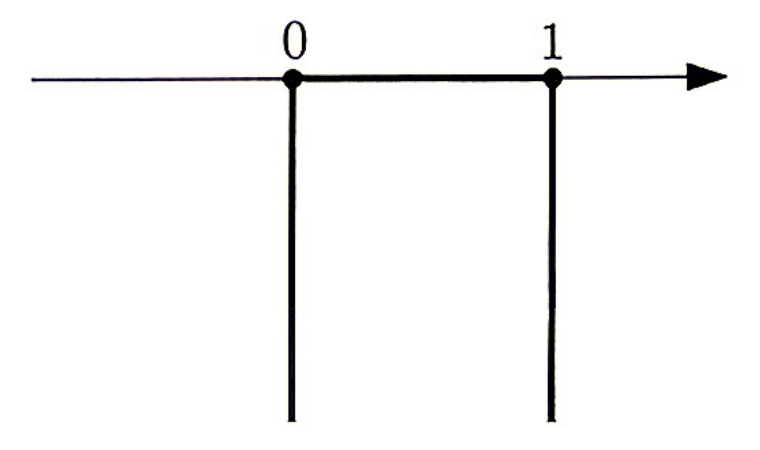
\includegraphics[width=0.50\linewidth]{figures/fig_p325_1.png}
  \caption*{图 10.7\quad $SS(\mathbf{k}_{(0,1]})$ 的示意图
  （原书 p.317, Figure 10.7）}
\end{figure}

\begin{wexer}{10.6.1}
仿照例 10.6.1 中的计算，计算奇性支撑
$SS(\mathbf{k}_{(0,1)})$、$SS(\mathbf{k}_{[0,1)})$ 与
$SS(\mathbf{k}_{[0,1]})$。
\end{wexer}

\begin{wrem}{10.6.4}
(i) 奇性支撑 $SS(\mathcal F)$ 常常是带角点的拉格朗日子集。判断子集是否为
拉格朗日的定义可以用泊松括号给出（参看例 2.3.2），因为经典的用辛结构给出的
定义会由于非光滑性而失效。
(ii) 按定义可以验证 $SS(\mathbf{k}_{\R})=0_{\R}\subset T^*\R$，它正是
$T^*\R$ 中的零截面（并与底流形 $\R$ 本身等同）。一般地，对任意光滑流形 $X$
有
\[
  SS(\mathbf{k}_X)=0_X\subset T^*X .
\]
(iii) 奇性支撑恢复了经典支撑 $\Op{supp}(\mathcal F)$（定义 10.2.6）的信息，
即
\[
  SS(\mathcal F)\cap 0_X=\Op{supp}(\mathcal F).
\]
\end{wrem}

\begin{wexer}{10.6.2}
给定范畴 $\Op{Sh}(\mathbf{k}_X)$ 中的正合列
$0\to\mathcal F_1\to\mathcal F_2\to\mathcal F_3\to0$，证明它们的奇性支撑满足
如下\textbf{三角不等式}：
(i) $SS(\mathcal F_2)\subset SS(\mathcal F_1)\cup SS(\mathcal F_3)$；
(ii) $SS(\mathcal F_i)\triangle SS(\mathcal F_j)\subset SS(\mathcal F_k)$，
其中 $i,j,k\in\{1,2,3\}$ 两两不同。这里 $A\triangle B$ 表示集合 $A$ 与 $B$
的\textbf{对称差}，即 $A\triangle B:=(A\setminus B)\cup(B\setminus A)$。
\end{wexer}

下面这个例子说明习题 10.6.2。

\begin{wexam}{10.6.3}
由于 $Z'=(0,1]\subset(0,2]=Z$ 在 $Z$ 中闭，由 (10.11)，在范畴
% >>> p326
$\Op{Sh}(\mathbf{k}_{\R})$ 中有
\[
  0\to\mathbf{k}_{(1,2]}\to\mathbf{k}_{(0,2]}
  \to\mathbf{k}_{(0,1]}\to0 .
\]
于是与例 10.6.2 类似，可以画出 $SS(\mathbf{k}_{(0,1]})$、
$SS(\mathbf{k}_{(1,2]})$ 与 $SS(\mathbf{k}_{(0,2]})$ 的示意图（见图 10.8）。
于是显然
\[
  SS(\mathbf{k}_{(0,2]})\subset
  SS(\mathbf{k}_{(0,1]})\cup SS(\mathbf{k}_{(1,2]})
\]
以及
\[
  SS(\mathbf{k}_{(0,1]})\triangle SS(\mathbf{k}_{(1,2]})
  \subset SS(\mathbf{k}_{(0,2]}),
\]
其中上述两个包含都是严格的。\hfill$//$
\end{wexam}

\begin{figure}[htbp]
  \centering
  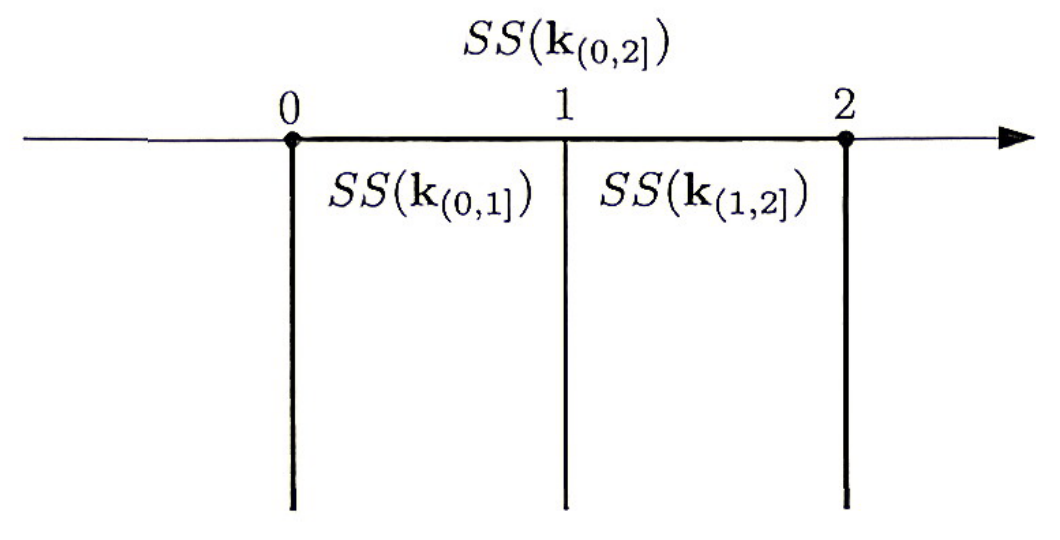
\includegraphics[width=0.68\linewidth]{figures/fig_p326_1.png}
  \caption*{图 10.8\quad $SS(\mathbf{k}_{(0,1]})$、
  $SS(\mathbf{k}_{(1,2]})$ 与 $SS(\mathbf{k}_{(0,2]})$ 的示意图
  （原书 p.318, Figure 10.8）}
\end{figure}

为计算更一般的子集 $Z\subset X$ 对应的层 $\mathbf{k}_Z$ 的奇性支撑，我们需要
经典的定义——余法丛；事实上，我们在例 3.4.4 中已见过它的一个特殊情形。

\begin{wdefn}{10.6.3}
设 $Z\subset X$ 是 $X$ 的光滑子流形，则 $Z$ 在 $X$ 中的
\textbf{余法丛}（conormal bundle）定义为
\[
  \nu^*_ZX=\bigl\{(z,p)\in T^*X\ \big|\ z\in Z,\
  \text{且}\ p|_{T_zZ}=0\bigr\}.
\]
可以数出 $\nu^*_ZX$ 的维数：若 $\dim(Z)=m\le n=\dim X$，则
\[
  \dim\nu^*_ZX=m+(n-m)=n=\frac12\dim T^*X,
\]
它恰好是 $T^*X$ 维数的一半。事实上，每个余法丛都是 $T^*X$ 的拉格朗日子流形
（习题）。
\end{wdefn}

% [Tutor Note: 易错预警——余法丛 $\nu^*_ZX$ 由「$p$ 在 $T_zZ$ 上为零」定义，
% 其纤维是 $T_zZ$ 的零化子（annihilator），维数为 $n-m$；不要把它与法丛
% $N_ZX=TX/TZ$（维数 $n-m$，但为商丛而非子丛）混淆。$\nu^*_ZX$ 是
% $T^*X$ 的拉格朗日子流形，这是例 3.4.4 中「单位余法丛是勒让德子流形」的
% 辛几何对应物：前者是后者的锥化（把单位余法丛沿纤维方向取正锥）。]

\begin{wexam}{10.6.4}
(i) 若 $Z=X$，则对任意 $z\in X$ 有 $p|_{T_zZ}=0$，从而 $p=0$。因此
$\nu^*_XX=0_X$。
(ii) 若 $Z$ 是一个点 $z$，则 $T_zZ=0$，这意味着对 $p$ 没有限制。因此
$\nu^*_zX$ 就是纤维 $T^*_zX$。\hfill$//$
\end{wexam}

% >>> p327
下述命题使我们能计算一大类形如 $\mathbf{k}_Z$（$Z\subset X$ 为子流形）的层
的奇性支撑。更多细节见 [135] 的 §5.3。

\begin{wprop}{10.6.1}（[135] 中命题 5.3.2）
设 $Z\subset X$ 是满足 $\operatorname{codim}(Z)\ge1$ 的子流形，则
$SS(\mathbf{k}_Z)=\nu^*_ZX$。
\end{wprop}

上述命题还表明：$T^*X$ 中的拉格朗日子流形——余法丛 $\nu^*_ZX$——有层对应物
$\mathbf{k}_Z$，二者通过奇性支撑 $SS$ 相联系。下一个问题是自然的后续。

\begin{wque}{10.6.1}
给定 $T^*X$ 中的拉格朗日子流形 $L$（$X$ 紧），是否存在层
$\mathcal F\in\Op{Ob}(\Op{Sh}(\mathbf{k}_X))$ 使得 $SS(\mathcal F)=L$？
\end{wque}

注意，由于 $SS(\mathcal F)$ 的锥性（见 (10.34) 下方的段落），上述问题只有在
知道如何「锥化」$L$ 之后才有意义。我们在下面的例子中探讨这一点。

\begin{wexam}{10.6.5}
设 $f:X\to\R$ 是光滑函数。考虑 $\dd f$ 的图
\[
  \mathrm{graph}(\dd f)
  =\bigl\{(x,\dd f(x))\in T^*X\ \big|\ x\in X\bigr\}.
\]
我们想构造一个层，使其奇性支撑能恢复这个图 $\mathrm{graph}(\dd f)$。巧妙的
一步是转到空间 $X\times\R$，并考虑如下区域：
\begin{equation}\tag{10.35}
  N_f:=\bigl\{(x,t)\in X\times\R\ \big|\ f(x)+t\ge0\bigr\},
\end{equation}
其中 $t$ 记录 $f$ 在 $X$ 上的取值。然后考虑
$\mathbf{k}_{N_f}\in\Op{Ob}(\Op{Sh}(\mathbf{k}_{X\times\R}))$，我们要计算
$SS(N_f)\subset T^*(X\times\R)$。

注意上面的命题 10.6.1 不能直接应用，因为 $N_f\subset X$ 是闭区域
（余维为 $0$）。一般地，模仿定义 10.6.3 中的余法丛 $\nu^*_ZX$，当 $Z$ 是
$X$ 的闭区域（可以有光滑边界）时，可如下定义 $Z$ 的余法丛：
\begin{align*}
  \nu^*_ZX
  &:=\bigl\{(z,0)\in T^*X\mid z\in\operatorname{int}(Z)\bigr\}
   \cup\bigl\{(z,p)\in T^*X\mid z\in\partial Z,\ p|_{T_z\partial Z}=0\bigr\}\\
  &=\bigl\{(z,0)\in T^*X\mid z\in Z\bigr\}
   \cup\bigl\{(z,p)\in T^*X\mid z\in\partial Z,\ p(n(z))>0\bigr\}\\
  &\qquad\cup\bigl\{(z,p)\in T^*X\mid z\in\partial Z,\ p(n(z))<0\bigr\},
\end{align*}
其中 $n(z)$ 表示 $z\in\partial Z$ 处的\textbf{外指}单位法向量。于是我们有
下述命题。

\begin{wprop}{10.6.2}
若 $Z\subset X$ 是闭区域，则
\[
  SS(\mathbf{k}_Z)=\bigl\{(z,0)\in T^*X\mid z\in Z\bigr\}
  \cup\bigl\{(z,p)\in T^*X\mid z\in\partial Z,\ p(n(z))<0\bigr\},
\]
它与上面 $\nu^*_ZX$ 的定义一致。若 $Z\subset X$ 是开区域，则
\[
  SS(\mathbf{k}_Z)
  =\overline{\bigl\{(z,0)\in T^*X\mid z\in Z\bigr\}}
  \cup\bigl\{(z,p)\in T^*X\mid z\in\partial Z,\ p(n(z))>0\bigr\}.
\]
\end{wprop}

% [Tutor Note: 原文疑误——命题 10.6.2（以及本节前面闭区域余法丛的第二行）
% 中只写了 $p(n(z))>0$ 或 $p(n(z))<0$，但按余法丛的定义还应同时要求
% $p|_{T_z\partial Z}=0$（即 $p$ 沿法向），否则该集合会包含大量带切向分量的
% 余向量，维数也大于 $\dim X$。正确读法是 $p=c\,n(z)$（$c>0$ 或 $c<0$）。
% 亦可用图 10.9 校对符号：对 $Z=(-\infty,1]$，外法向 $n>0$，图中竖线朝
% $p<0$，即 $p(n(z))<0$。已记入 review_ch10b.md。]

作为快速例子，取 $X=\R$，$Z=(-\infty,1]\subset\R$ 或 $Z=(0,\infty)$，则
$SS(\mathbf{k}_{(-\infty,1]})$ 与 $SS(\mathbf{k}_{(0,\infty)})$ 如图 10.9
所示。

% >>> p328
\begin{figure}[htbp]
  \centering
  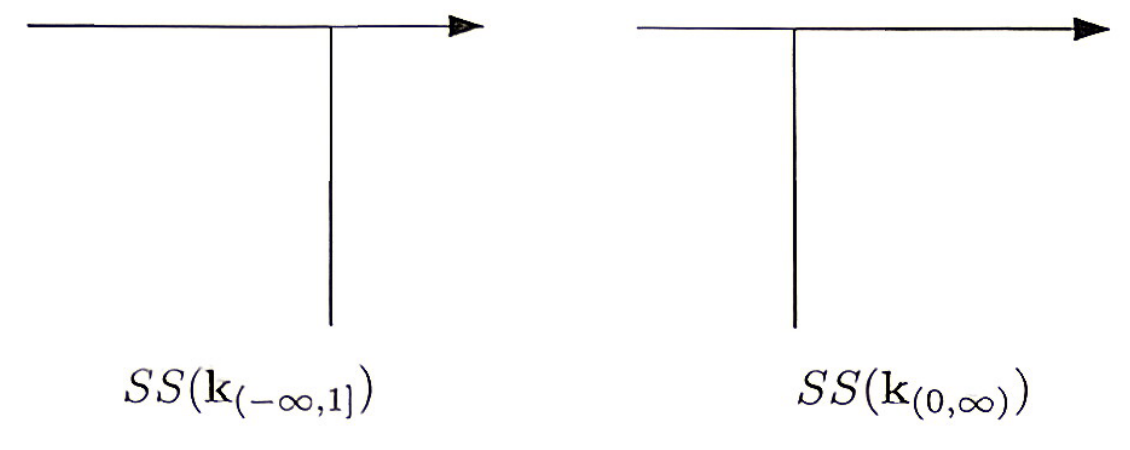
\includegraphics[width=0.78\linewidth]{figures/fig_p328_1.png}
  \caption*{图 10.9\quad $SS(\mathbf{k}_{(-\infty,1]})$ 与
  $SS(\mathbf{k}_{(0,\infty)})$ 的示意图
  （原书 p.320, Figure 10.9）}
\end{figure}

回到 $N_f$ 与 $SS(N_f)$ 的计算。由于 $N_f$ 是 $X\times\R$ 的闭区域，由命题
10.6.2 的第一个结论有
\begin{align*}
  SS(N_f)
  &=0_{N_f}\cup\Bigl\{((x,p),(t,\tau))\in T^*X\times T^*\R
   \ \Big|\ (x,t)\ \text{满足}\ f(x)+t=0,\
   \text{且}\ p\ \text{指向内部}\Bigr\}\\
  &=0_{N_f}\cup\bigl\{(x,\tau\dd f(x),-f(x),\tau)
   \ \big|\ x\in X,\ \tau>0\bigr\}.
\end{align*}
由 $SS(N_f)\subset T^*(X\times\R)$，可作如下约化：忘掉零截面
$0_{N_f}$，再把 $(x,p,t,\tau)$ 投影为
$(x,p/\tau)\in T^*X$。这恰好把 $SS(N_f)\setminus0_{N_f}$ 映满
$\mathrm{graph}(\dd f)$。因此，(10.35) 中定义的
$N_f\in\Op{Ob}(\Op{Sh}(\mathbf{k}_{X\times\R}))$ 正是拉格朗日子流形
$\mathrm{graph}(\dd f)\subset(T^*X,\omega_{\mathrm{can}})$ 的层对应物。本例
到此结束。\hfill$//$
\end{wexam}

回忆 §10.1 中「生成函数」推广了 $\mathrm{graph}(\dd f)$。设 $L\subset T^*X$
容许生成函数（例如满足定理 10.1.1 中条件的那些 $L$），则按定义存在函数
$S:X\times\R^k\to\R$（对某个 $k\in\N$），使得
\begin{equation}\tag{10.36}
  L=\Bigl\{\Bigl(x,\frac{\partial S}{\partial x}(x,e)\Bigr)\in T^*X
  \ \Big|\ \frac{\partial S}{\partial e}(x,e)=0\Bigr\}.
\end{equation}
遵循与 (10.35) 相同的精神，考虑如下层：
\begin{equation}\tag{10.37}
  N_S:=\bigl\{(x,e,t)\in X\times\R^k\times\R
  \ \big|\ S(x,e)+t\ge0\bigr\}.
\end{equation}
为去掉 (10.37) 中的欧氏空间 $\R^k$，应用自然投影
$p:X\times\R^k\times\R\to X\times\R$。于是按如下过程
\[
  \mathbf{k}_{N_S}\in\Op{Ob}(\Op{Sh}(\mathbf{k}_{X\times\R^k\times\R}))
  \xrightarrow{\ p_!\ }p_!\mathbf{k}_{N_S}
  \in\Op{Ob}(\Op{Sh}(\mathbf{k}_{X\times\R}))
  \xrightarrow{\ SS\ }SS(p_!\mathbf{k}_{N_S}),
\]
便得到奇性支撑 $SS(p_!\mathbf{k}_{N_S})\subset T^*(X\times\R)$。这里我们使用
固有前推 $p_!$（定义于 (10.19)），而不用前推 $p_*$，因为所讨论的空间含有
非紧分量 $\R$（以及 $\R^k$），而在那里紧支截面通常表现更好。然后，按照例
10.6.5 末尾引入的同一约化过程，可以把 $SS(p_!\mathbf{k}_{N_S})$ 转化为
(10.36) 中定义的拉格朗日子流形 $L\subset T^*X$。

下面是一个说明上述过程的初等例子。

% >>> p329
\begin{wexam}{10.6.6}
取 $X=\R$ 与 $L=0_{\R}\subset T^*\R\cong\R\times\R$。则 $L$ 可由函数
$S:\R\times\R\to\R$，$S(x,e)=e^2$ 生成，其中 $(x,e)\in\R\times\R$。由
(10.37) 有
\[
  N_S=\bigl\{(x,e,t)\in\R\times\R\times\R\ \big|\ e^2+t\ge0\bigr\}.
\]
然后考虑 $p_!\mathbf{k}_{N_S}\in\Op{Ob}(\Op{Sh}(\mathbf{k}_{\R\times\R}))$，
可以验证（习题）
\[
  p_!\mathbf{k}_{N_S}
  =\mathbf{k}_{\{(x,t)\in\R^2\mid t\ge0\}}
  =\mathbf{k}_{\R\times[0,\infty)},
\]
它约化为 $0_{\R}=L\subset T^*\R$。\hfill$//$
\end{wexam}

除拉格朗日子流形外，辛几何中另一个重要要素是哈密顿动力学，它由哈密顿函数
生成的哈密顿同痕所代表。遗憾的是，本书只能考虑 $(T^*X,\omega_{\mathrm{can}})$
上的哈密顿动力学。对于更一般的设定，例如某些闭辛流形，我们参考 Tamarkin
近期的工作 [212]（该工作迄今尚未被公众完全理解）。

设 $\Phi=\{\varphi^t_H\}_{t\in[0,1]}:[0,1]\times T^*X\to T^*X$ 是由哈密顿
函数 $H:[0,1]\times T^*X\to\R$ 生成的哈密顿同痕。回忆 $\Phi$ 的
\textbf{拉格朗日悬挂}（Lagrangian suspension，见定义 9.5.1）是
\[
  \Lambda_{\Phi}
  =\bigl\{\bigl(z,-\varphi^t_H(z),t,H_t(\varphi^t_H(z))\bigr)
  \ \bigl|\ (t,z)\in[0,1]\times T^*X\bigr\},
\]
它是 $T^*X\times T^*X\times T^*I$ 中的拉格朗日子流形，其中 $I=[0,1]$。我们
想得到 $\Lambda_{\Phi}$ 的层对应物，从而得到哈密顿同痕 $\Phi$ 的层对应物。
循例 10.6.5 中的同一思路，第一步是把 $\Lambda_{\Phi}$ 锥化：再添一个额外
空间 $\R$。

更确切地说，考虑新的哈密顿函数
$\widetilde H(t,(x,p)):I\times T^*X\times\dot T^*\R
(=T^*\R\setminus0_{\R})\to\R$，定义为
\[
  \widetilde H\bigl(t,(x,p),(s,\sigma)\bigr)
  :=\sigma H_t(x,p/\sigma).
\]
于是其哈密顿流有如下表达式：
\[
  \varphi^t_{\widetilde H}\bigl((x,p),(s,\sigma)\bigr)
  =\Bigl(\sigma\cdot\varphi^t_H(x,p/\sigma),
  \bigl(s+u(t,(x,p/\sigma)),\sigma\bigr)\Bigr),
\]
其中 $u(t,(x,p/\sigma))$ 是 $I\times T^*X$ 上的某个函数。注意这是
$T^*X\times T^*\R$ 上的 $\R_+$-齐次哈密顿微分同胚，即
\[
  \varphi^t_{\widetilde H}\bigl((x,\lambda p),(s,\lambda\sigma)\bigr)
  =\lambda\cdot\varphi^t_{\widetilde H}\bigl((x,p),(s,\sigma)\bigr),
\]
其中右端的「$\lambda$」表示在余向量上乘以 $\lambda$。这意味着，对扩张后的
哈密顿同痕
$\widetilde\Phi=\{\varphi^t_{\widetilde H}\}_{t\in I}$
（定义在 $\dot T^*(X\times\R)(=T^*(X\times\R)\setminus0_{X\times\R})$ 上），

% >>> p330
其拉格朗日悬挂
$\Lambda_{\widetilde\Phi}\subset T^*(X\times\R)\times T^*(X\times\R)
\times T^*I$ 是锥形拉格朗日子流形。

我们期待的拉格朗日子流形 $\Lambda_{\Phi}$ 的层对应物由下述著名结果给出。就
记号而言，下面定理中的 $M$ 即我们的 $X\times\R$，定理中的 $\Phi$ 即上面
构造的 $\widetilde\Phi=\{\varphi^t_{\widetilde H}\}_{t\in I}$。

\begin{wthm}{10.6.1}（Guillermou–Kashiwara–Schapira [106]）
给定紧流形 $M$，对任意 $\R_+$-齐次哈密顿同痕
$\widetilde\Phi:I\times\dot T^*M\to\dot T^*M$，存在对象
$\mathcal F(=\mathcal F^{\bullet})
\in\Op{Ob}(D(\Op{Sh}(\mathbf{k}_{M\times M\times I})))$，在同构意义下唯一，
满足如下性质：(i) 奇性支撑 $SS(\mathcal F)$（稍后将对导出范畴中的对象定义）
包含于 $\Lambda_{\widetilde\Phi}\cup0_{M\times M\times I}$；
(ii) $\mathcal F|_{t=0}\simeq\mathbf{k}_{\Delta}$，其中
$\Delta\subset M\times M$ 是 $M\times M$ 的对角线。
\end{wthm}

% [Tutor Note: 术语与含糊点拨——定理 10.6.1 中的对象
% $\mathcal F$ 称为哈密顿同痕 $\widetilde\Phi$（在 $\dot T^*M$ 上）的
% \textbf{GKS 层量子化}（GKS sheaf quantization），常记为
% $\mathcal K_{\Phi}$。条件 (i) 中的 $SS(\mathcal F)$ 对导出范畴对象
% $\mathcal F^{\bullet}$ 的定义需要 §10.7 的 $\Gamma_Z$ 与「传播」的推广；
% 条件 (ii) 则说明 $\mathcal F$ 在 $t=0$ 处退化为对角线上的常值层
% $\mathbf{k}_\Delta$，这正对应于「Hamiltonian 同痕在 $t=0$ 时为恒等」。]

\begin{wrem}{10.6.5}
除拉格朗日子流形与哈密顿同痕外，辛几何中另一个流行的要素是 Liouville 域。
得益于 Tamarkin 在 [213] 中的开创性工作，人们引入了范畴方法来建立
$(\R^{2n},\omega_{\mathrm{std}})$ 中 Liouville 域的层量子化，它与 §6.3 中
引入的辛同调有一些共同特征。更多细节见 [246] 的 §4.8。另一点要说明的是：
除例 10.6.5 中的那些拉格朗日子流形及其在 (10.36) 中的推广外，Viterbo
[238, 236] 与 Guillermou [105] 证明了 $T^*X$ 中任何紧的恰当拉格朗日子流形
都有层对应物（另见 Asano–Ike 近期的工作 [17]）。
\end{wrem}

\begin{wexer}{10.6.3}
设 $(X,g)$ 是闭黎曼流形，$H:T^*X\to\R$ 由 $H(x,p)=|p|_g$ 给出（它已经是
$T^*X\setminus0_X$ 上的齐次哈密顿函数，故无需作任何锥化/齐次化处理）。则对
足够小的 $\epsilon>0$（例如小于 $(X,g)$ 的单射半径），考虑如下集合
\[
  Z:=\bigl\{(x,y,t)\in X\times X\times(-\epsilon,\epsilon)
  \ \big|\ d(x,y)\le t\bigr\}
\]
以及层 $\mathbf{k}_Z$。证明 $SS(\mathbf{k}_Z)$ 满足：(i)
$(\mathbf{k}_Z)|_{t=0}\simeq\mathbf{k}_{\mathrm{var}\,\Delta}$，其中
$\Delta\subset X\times X$ 表示对角线；(ii)
$SS(\mathbf{k}_Z)\subset\Lambda_{\Phi_H}\cup0_{X\times X\times(-\epsilon,\epsilon)}$，
其中 $\Lambda_{\Phi_H}$ 表示由 $H$ 生成的哈密顿同痕的拉格朗日悬挂，具体为
\[
  \Lambda_{\Phi_H}
  =\bigl\{\bigl((x,p),-\varphi^t_H(x,p),(t,-H(x,p))\bigr)
  \ \big|\ (x,p)\in T^*X\bigr\}.
\]
因此 $\mathbf{k}_Z$ 是 $\Phi_H$ 的 GKS 层量子化。这是 GKS 层量子化的最早的
非平凡例子之一。
\end{wexer}
